
%
%  $Description: Author guidelines and sample document in LaTeX2e$
%
%  $Author: ienne, paulley $
%  $Date: 2002/04/15 11:20:59 $
%  $Revision: 1.0 $
%

\documentclass{ieee}

%------------------------------------------------------------------------- 
% 
% Use \documentclass[pagenumbers]{ieee}
%
% to produce page numbers, bottom centered, in the output. Default is 
% no page numbers for camera-ready copy.
%
%------------------------------------------------------------------------- 

\usepackage{times}
\usepackage[latin1]{inputenc}
\usepackage[english]{babel}
\usepackage{graphicx,url}
\usepackage{titlesec}



\begin{document}

\title{A short study of the addition of an L4 cache memory\\ with interleaved cache hierarchy to multicore architectures}

\author{Carlos Eduardo B. Bezerra, Cl�udio F. R. Geyer\\
Institudo de Inform�tica\\
Universidade Federal do Rio Grande do Sul\\
Av. Bento Gon�alves, 9500, Porto Alegre, RS\\
\{carlos.bezerra, geyer\}@inf.ufrgs.br\\
% For a paper whose authors are all at the same institution,
% omit the following lines up until the closing ``}''.
% Additional authors and addresses can be added with ``\and'',
% just like the second author.
% \and
% Second Author\\
% Institution2\\
% First line of institution2 address\\ Second line of institution2 address\\ 
% SecondAuthor@institution2.com\\
}

\maketitle
\thispagestyle{empty}

\begin{abstract}
%After a certain stagnation of the processor clock increase rate, it has been invested in multicore architectures to meet the demand for processing capacity required by applications increasingly heavy. These applications have a requirement for increased storage space in main memory, which requires a proportional increase in the processor cache memory. However, just increasing cache memory to a processor can not only not increase its performance, but also reduce its efficiency by increasing the memory access time.
In this work, a comparison is made between the performance of a multicore architecture with a large L3 cache and an architecture with an additional cache memory level, L4. It is also proposed an architecture with an interleaved cache hierarchy, for reducing the memory search depth when two cores share a variable. It was found that a better structured memory with four levels hierarchy performed the simulated tasks in less time than an architecture with a large L3 cache. Finally, it has been shown that interleaving the cache hierarchy may bring significant benefits.
\end{abstract}



%------------------------------------------------------------------------- 
\section{Introduction}

In the past few years, due to a stagnation of the processor clock frequency \cite{zhao1008scs}, manufacturers have opted for the production of processors with multiple processing cores -- or multicore processors. Examples are the architectures of Intel (\emph{Dunnington}, \emph{Nehalem} etc.), AMD (\emph{Barcelona}, \emph{Budapest}, \emph{Deneb} etc.) and Sun (\emph{Niagara}, \emph{Victoria Falls} etc.).

	
The cache are used to reduce the number of latency cycles that a processor must wait to access a given memory block. Reducing the number of cycles, it reduces the time required to access the data. For this reason, the time to access data in the cache memory is considerably shorter than the time required to access the main memory, for example.

However, recent applications have an increasingly large volume of data to process. This large amount of data, if not accessed quickly by the processing unit, can lead to a poor system performance \cite{li98fem}. Another issue is that in multicore architectures, multiple cores may be using the memory at the same time. Because of these reasons, it is recommendable to increase the size of the cache (which is faster) at the proportion of the increase of application data and the number of processor cores.

The question is that the simple increase of the cache may not be sufficient to reduce the execution time of tasks performed by the processor. Actually, a careless increase of the memory size may even reduce the speed of the system. This happens because the larger the memory, the greater the time of access, due to a more complex structure of addressing \cite{goodman98ucm}. Moreover, if several cores are trying to access the memory at the same time, there will be a contention for the access to the bus to that memory, so that one or more processors have to wait until the bus is released. A poor structure design for the cache memory may lead an architecture with more memory to be slower than an architecture with less memory, but with a more efficient structure

Considering these aspects, this work has done a study of the influence of the cache structure in multicore processors, comparing the performance of a hierarchy with 3 memory levels to two other hierarchies, each with 4 levels, introducing an L4 cache shared between all cores. As a contribution, this work proposed and tested an interleaved memory hierarchy -- which will be described in the next sections -- with the objective of reducing the depth of the search that a core must perform to get the latest value of a shared variable.

The text is organized as follows: in section \ref{sec:prop}, we describe in more detail the proposal of this work, including the idea of interleaving the hierarchy of the cache memory; in section \ref{sec:simul}, we present the details of modeling and the parameters of the simulations carried out; in section \ref{sec:result}, we show the results and a brief analysis and, in section \ref{sec:conc}, the conclusions of this work are presented.

%------------------------------------------------------------------------- 
\section{Proposal}
\label{sec:prop}
	
This study had two goals, which are: seek evidence that the addition of a fourth level of cache memory is more beneficial than increasing the L3 cache and evaluate the performance gain that is achieved by interlacing the hierarchy of cache memories. To examine the difference in performance with a large L3 cache, compared to the addition of an L4 cache memory module, we compared the following architectures:

\begin{itemize}
 \item a multicore architecture, simlar to the Dunnington architecture used in Intel Xeon, which had eight cores, with four modules of L2 cache, each shared by a pair of cores, and a large L3 memory (with 32 megabytes of space), shared among all eight cores;% (Figure \ref{L3});
\end{itemize}

% \begin{figure}[!h]
%   \centering  
%   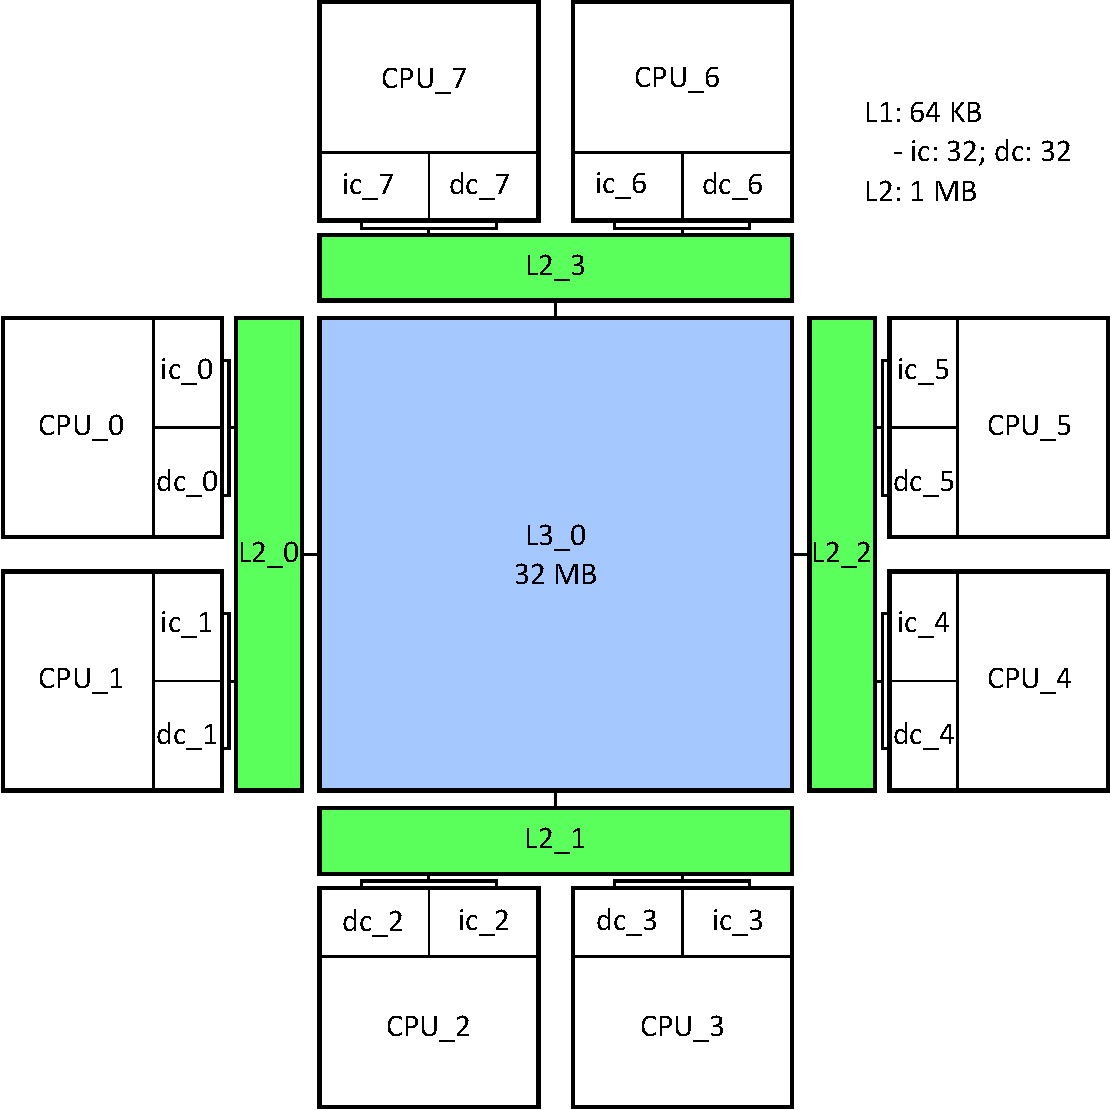
\includegraphics[width=0.8\linewidth]{images/arq_L123.pdf}
%   \caption{Architecture with three cache levels}
%   \label{L3}
% \end{figure}

\begin{itemize} 
\item a multicore architecture, similar to the previous one, also with eight cores, but the 32 megabytes of L3 memory were divided into: two 8 megabytes L3 memory modules, each shared by half of the cores, and a 16 megabytes L4 memory, shared by all cores;% (Figure \ref{L4}).
\end{itemize}

% \begin{figure}[!h]
%   \centering  
%   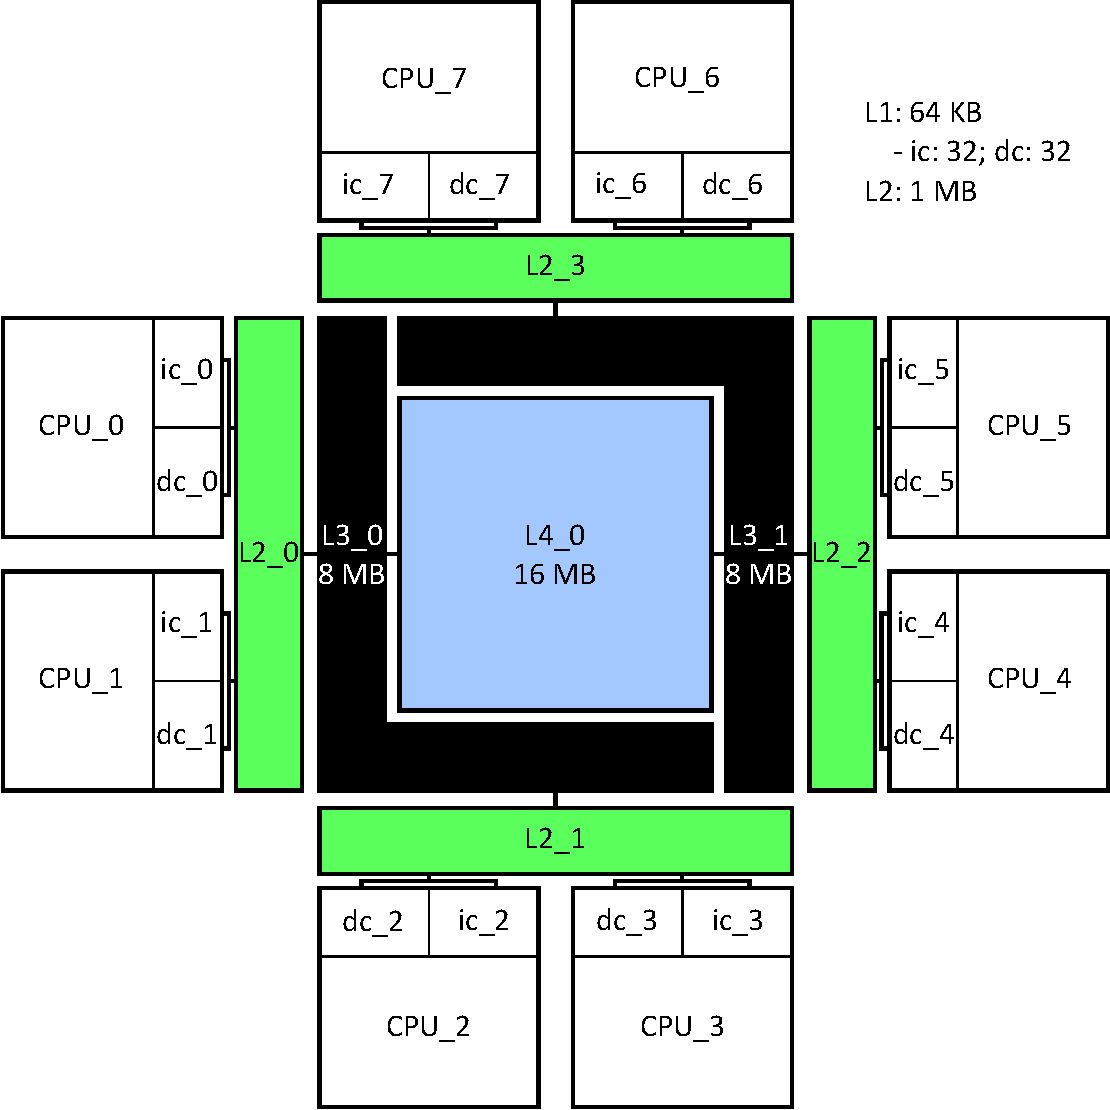
\includegraphics[width=0.8\linewidth]{images/arq_L1234.pdf}
%   \caption{Architecture with four cache levels}
%   \label{L4}
% \end{figure}

Another contribution of this work was also the proposal of an hierarchy interleaving of the hierarchy of cache memories. To get a result indicating whether there is any benefit by using this kind of approach, we compared the following architectures:

\begin{itemize}
 \item an architecture with four cache levels (L1, L2, L3 and L4), where each module has only one lower level cache module in the memory hierarchy;
\end{itemize}

\begin{itemize}
 \item another architecture, in which each L2 cache module can be linked to one or two memories in the L3 level of the hierarchy. Figure \ref{L4Interleaved} illustrates the interleaved memory hierarchy architecture.
\end{itemize}

\begin{figure}[!h]
  \centering  
  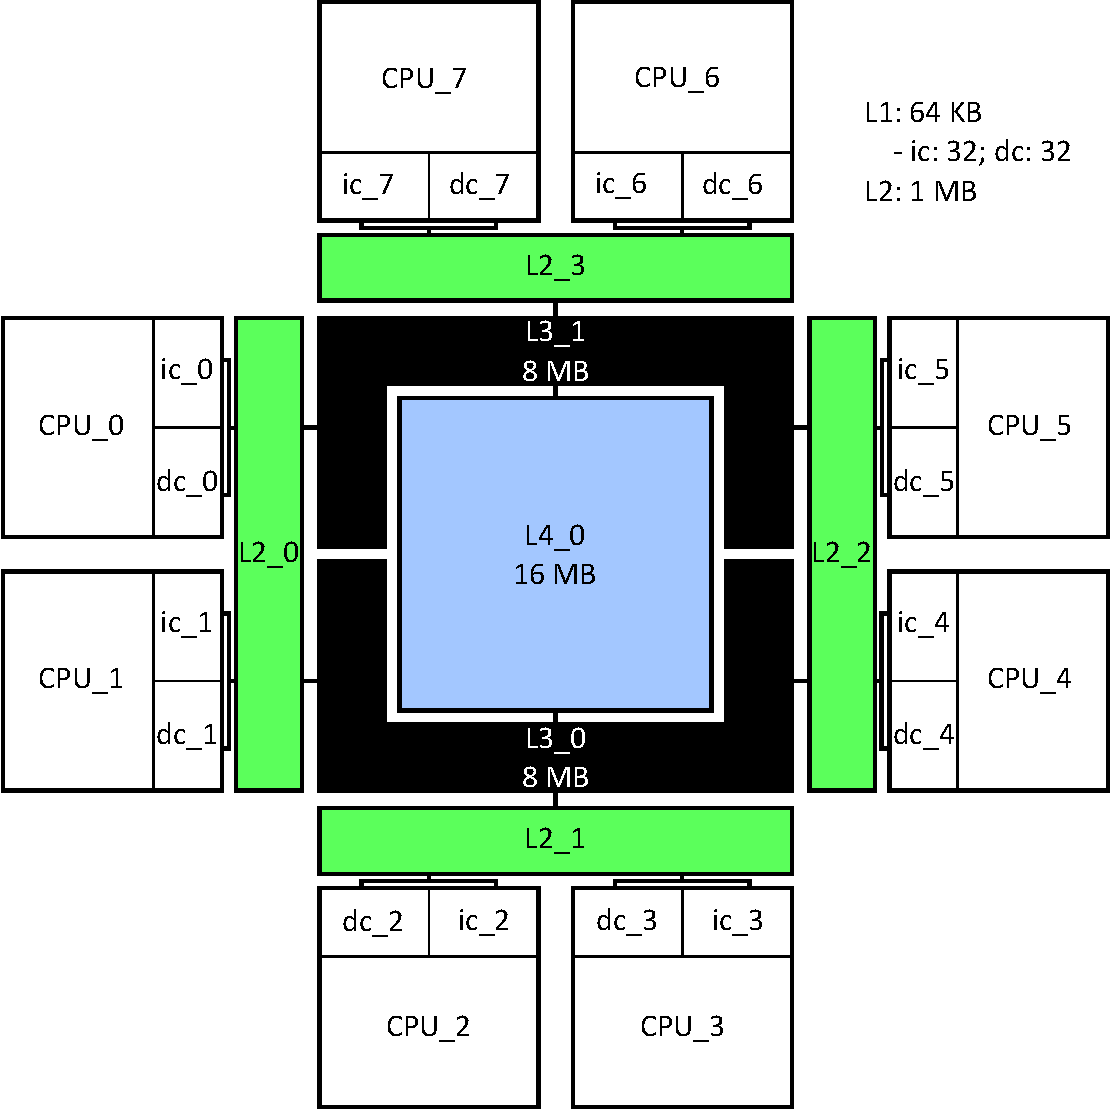
\includegraphics[width=0.8\linewidth]{images/arq_L1234Interleaved.pdf}
  \caption{Architecture with four cache levels and interleaved hierarchy}
  \label{L4Interleaved}
\end{figure}

% \begin{figure}[!h]
%   \centering  
%   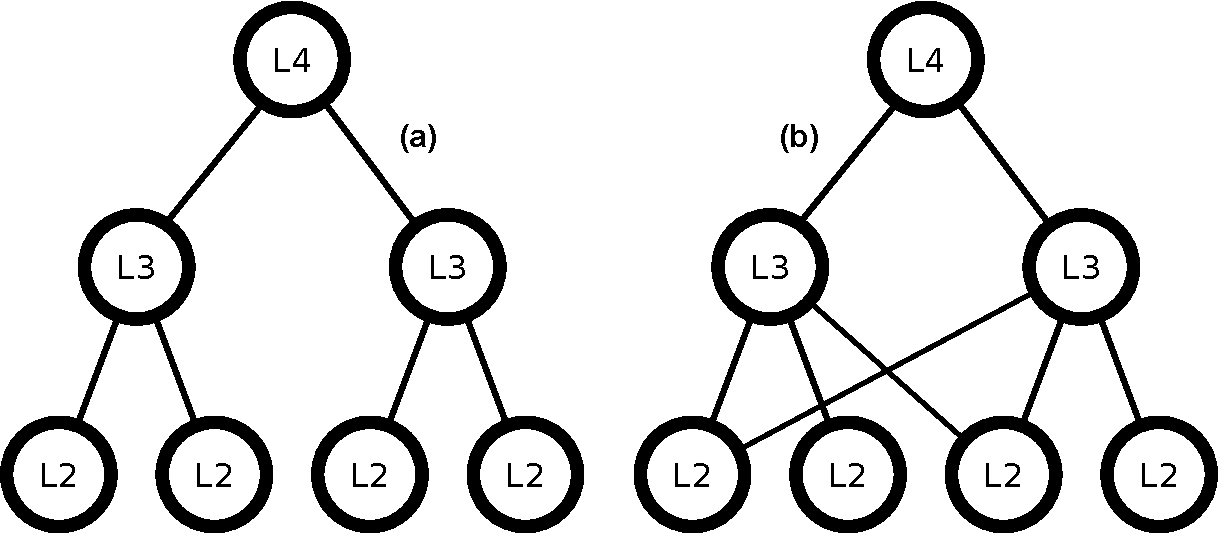
\includegraphics[width=0.8\linewidth]{images/treescompare}
%   \caption{Trees representing the evaluated hierarchies}
%   \label{treescompare}
% \end{figure}

The objective of this interleaving is to reduce the problem of having to perform very deep searches in the cache memory hierarchy when two processing cores share a variable. Consider a situation in which the cores \emph{CPU\_0} and \emph{CPU\_7}, whose only common cache memory block is the L4 one, read and write the same variable \emph{x}. Without interleaving, when \emph{CPU\_0} writes in the variable, the value stored in the L1 cache of \emph{CPU\_7} would be incoherent and it would have to search the cache until the first memory area common to both cores -- in this case the L4 memory, which is more distant from the cores and probably has a longer access latency, reducing the system performance.

However, considering the architecture with interleave hierarchy shown in Figure \ref{L4Interleaved}, it would be enough to have the up-to-date value of \emph{x} stored in the third level cache \emph{L3\_1}. This way, it would not be necessary to perform a deep four levels search. Using this approach reduces the average search depth necessary for the cores to share data in cache memories. However, this mechanism has some details to be considered in a real implementation of the architecture. For example, when a \emph{cache-miss} occurs in a L2 cache, it may be necessary to search in two L3 caches -- in the example of Figure \ref{L4Interleaved}, this happens when a there is a cache miss in modules \emph{L2\_0} and \emph{L2\_2}. This may cause a longer access time, if the searches are sequential, or in a higher cost of manufacturing the hardware, if there is in the processor an unit responsible for conducting two searches in parallel and, when a result is found by one of them, returning it and aborting the other search.

In the following section, we present the details of the modeling of the proposed architectures and the tests performed with simulation.

%------------------------------------------------------------------------- 
\section{Modeling and simulation}
\label{sec:simul}

To perform the simulation of the architectures proposed in section \ref{sec:prop}, we used the Simics simulator \cite{magnusson2002sfs} (version 4). With Simics, one can model and simulate different computer architectures and run popular operating systems -- such as Linux -- on them. To model the architecture and hardware components, the Simics reads files written in a device modeling language (MLD), which lets you create components, set their attributes and connect them together. Once the operating systems was installed and configured, a program to assess performance -- NAS (\emph{Numerical Aerodynamic Simulation}) -- was installed to perform evaluations of the performance of the computer architectures via extensive numerical calculations \cite{bailey1995npb}.

The modeling of the proposed architectures was based on a sparc64 architecture (TI UltraSPARC II -- \textit{Blackbird}). All the modeled architectures have the following characteristics in common: 8 processing cores (168 MHz each); L1 cache: 64 KB; L1 latency: 2 cycles; L2 cache: 1 MB (each 1 MB module shared by two cores); L2 latency: 5 cycles.

The \textbf{L123} architecture has also a shared L3 cache of 32 MB for all cores, with 30 cycles latency. The \textbf{L1234} architecture, in turn, has two 8 MB L3 cache modules (each shared by four cores), with 15 cycles latency and one 16 MB L4 cache shared by all cores, with 30 cycles latency. Finally, the \textbf{L4Interleaved} architecture is very similar to the L1234 one, except that each L3 module is shared by a different set of cores, interleaving the cache levels. Also, the L3 latency is of 20 cycles.

The reasons for us to decide these parameters were: in L123 architecture, the L3 cache has 32 megabytes of size, causing an access time (30 cycles) higher than in L1234 architecture (15 cycles), where each L3 cache has only 8 megabytes. In L4Interleaved, each cache miss in L2 cache may require two searches in the L3 caches. To simulate this behavior, we set up the L3 access time to 20 cycles, as an estimate of average access time.

The operating system that was installed on each of the architectures simulated was Ubuntu (GNU/Linux, kernel 2.6.15-53). The software used for evaluation of the architectures, NAS, consists of several programs to assess performance. Two of them are the \textbf{BT} and the \textbf{CG}. Details about them can be found in \cite{bailey1995npb} and \cite{jin1999oip}.

%For each tested combination (architecture $\times$ assessment program), the test was repeated three times, due to restrictions in the time we had available to perform the tests. On the average, each repetition of the simulation took three hours. It is estimated that, even by running only three times each simulation, it has taken 54 hours. The next section will present the results with the simulations that were performed.

%------------------------------------------------------------------------- 
\section{Results}
\label{sec:result}

Both CG and BT seek to stress the components of processing and memory. BT has a higher execution time, allowing the evaluation of the processor, while CG aims to stress the memory, allowing us to test the performance of the simulated cache structure. OpenMP implementations \cite{dagum1998ois} of both programs were used in our tests. To collect data, it was used the \emph{magic instruction} from Simics, which allows to pause the simulation and extract the state of each component of hardware. The values measured with this method, for each program run (BT and CG) were: cpu cycles, cpu steps, and L3 and L4 read/write miss.

\begin{figure}[!h]
  \centering  
  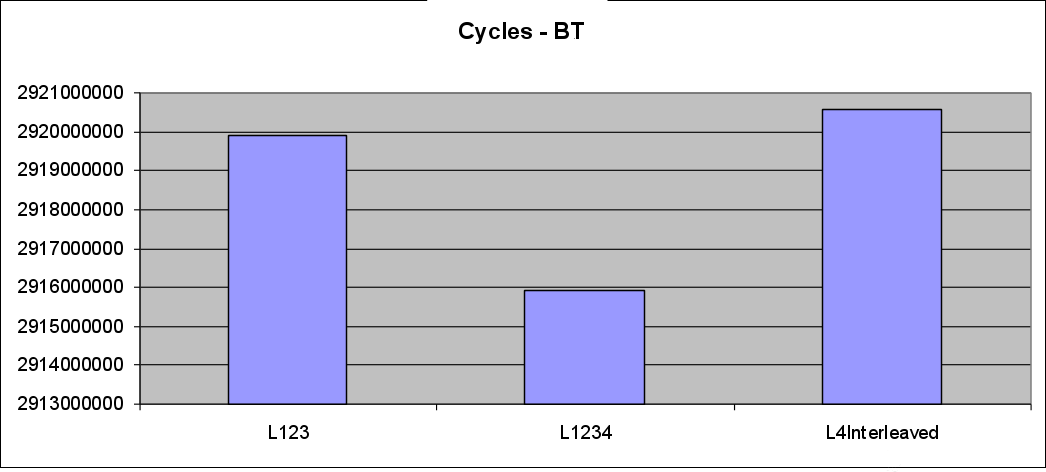
\includegraphics[width=\linewidth]{images/ciclos_bt.png}
  \caption{Cycles necessary to run BT}
  \label{ciclos_bt}
\end{figure}

\begin{figure}[!h]
  \centering  
  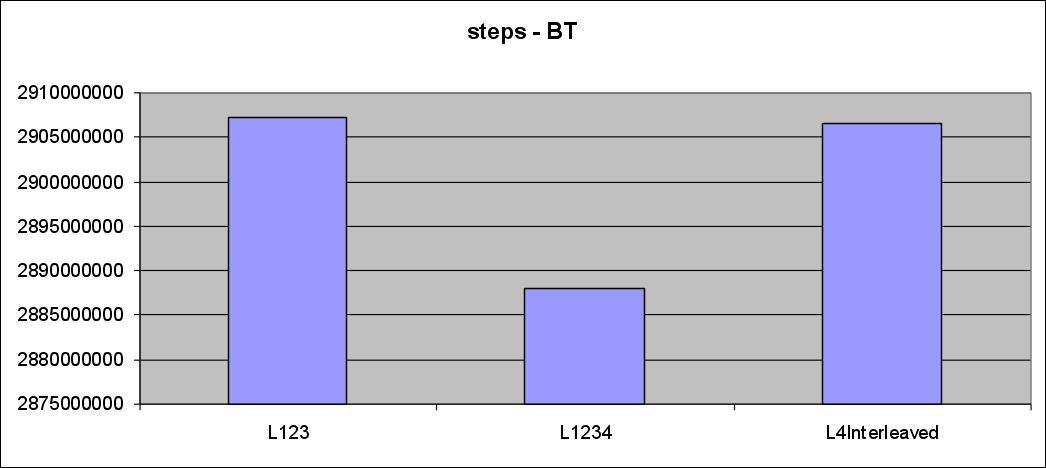
\includegraphics[width=\linewidth]{images/steps_bt.png}
  \caption{Steps necessary to run BT}
  \label{steps_bt}
\end{figure}

\begin{figure}[!h]
  \centering  
  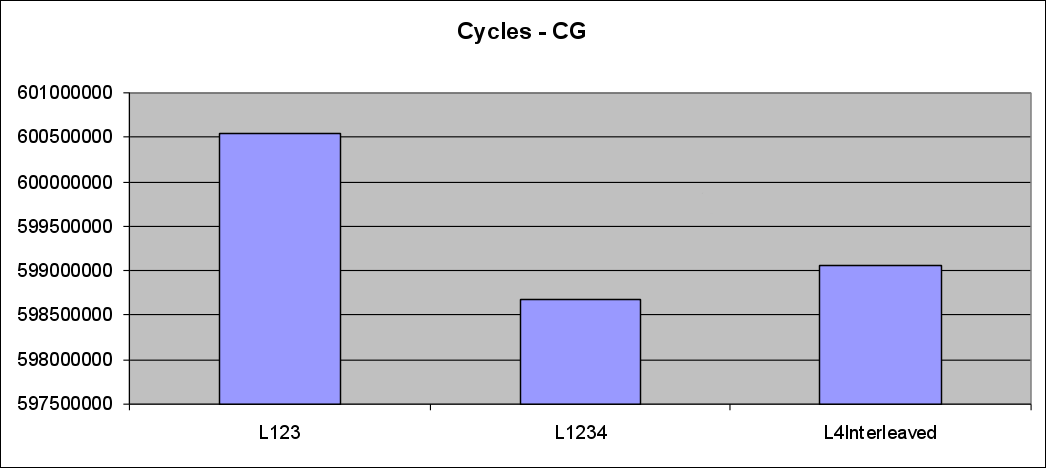
\includegraphics[width=\linewidth]{images/ciclos_cg.png}
  \caption{Cycles necessary to run CG}
  \label{ciclos_cg}
\end{figure}

\begin{figure}[!h]
  \centering  
  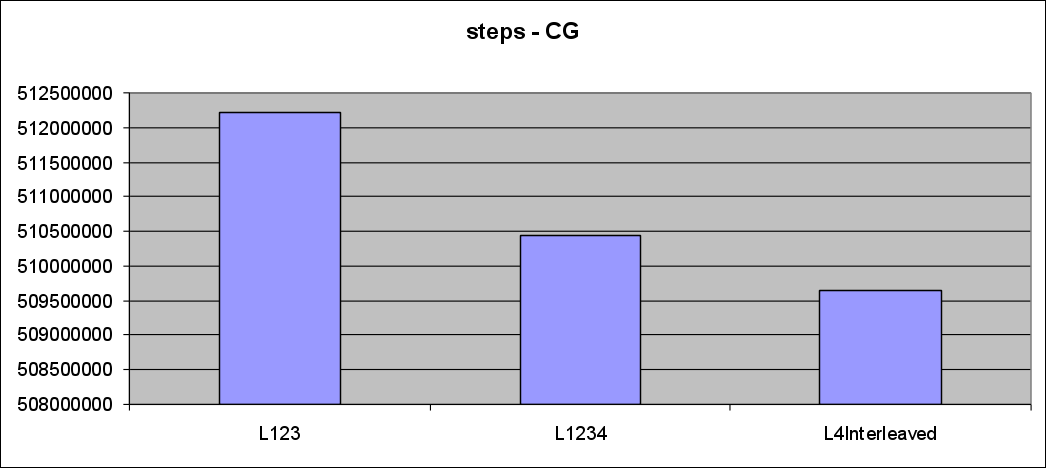
\includegraphics[width=\linewidth]{images/steps_cg.png}
  \caption{Steps necessary to run CG}
  \label{steps_cg}
\end{figure}

\begin{figure}[!h]
  \centering  
  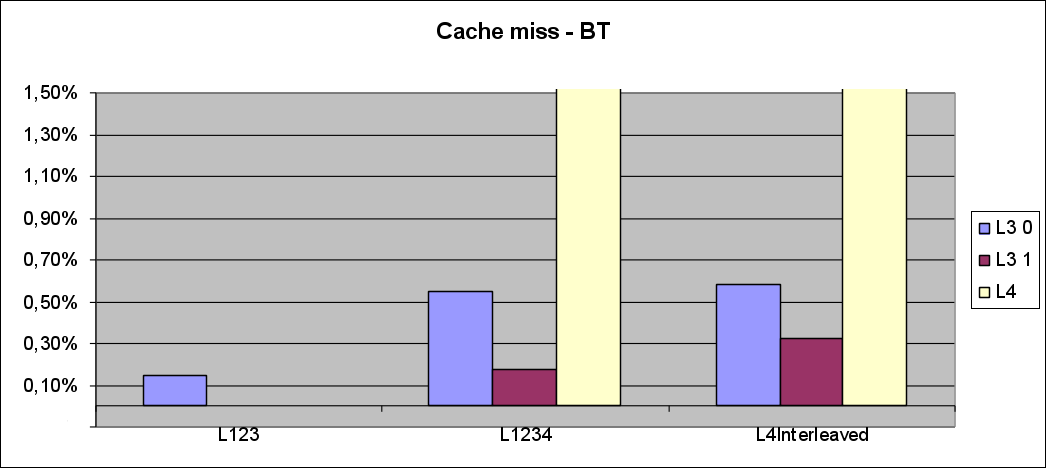
\includegraphics[width=\linewidth]{images/cachemiss_bt.png}
  \caption{Cache miss rate when running BT}
  \label{cachemiss_bt}
\end{figure}

\begin{figure}[!h]
  \centering  
  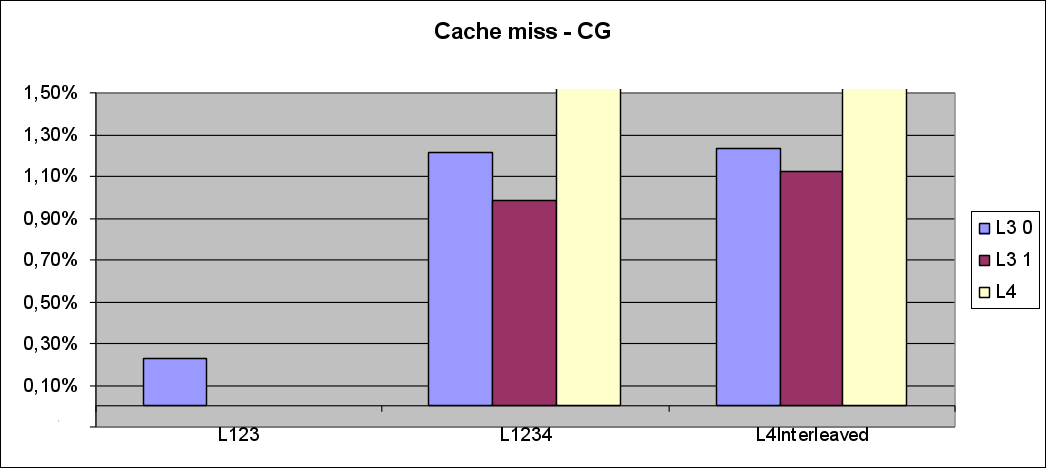
\includegraphics[width=\linewidth]{images/cachemiss_cg.png}
  \caption{Cache miss rate when running CG}
  \label{cachemiss_cg}
\end{figure}

Before analyzing the results, it must be considered that the standard deviation of the number of cycles did not exceed, in any of the tests, the value of 1000 (0.0001\%). Also, the standard deviation of the number of steps did not exceed the value of 1000000 (0.1\%). Taking this into account, we consider as relevant the result differences  found in the graphs presented.

In the graphs of Figure \ref{ciclos_bt} and Figure \ref{steps_bt}, we can see that there was a significant difference in the number of cycles and steps when running BT on the different architectures. The architecture L1234 had the lowest execution time, probably due to a lower contention to access each L3 cache (four processors, instead of eight) in addition to a shorter access time (8 MB, instead of 32). Even with a four times smaller L3 cache module than L123, apparently the lower contention and shorter access time were crucial for a faster execution. The architecture L4Interleaved had an execution time close to L123, probably due to its longer access time to the L3 cache.

Figure \ref{ciclos_cg} and Figure \ref{steps_cg} show a more interesting behaviour: both architectures with L4 cache had better performance than that without the fourth level, but the number of cycles of L4Interleaved is slightly higher than L1234, while the number of steps is lower. The most likely cause for this is the interleaving of the hierarchy cache. Probably, the number of accesses to the memory in L4Interleaved is smaller. However, as each access to the L3 has a higher cost, the number of cycles ended up being higher. Probably in this case it would be better to have in the processor an unit responsible for performing the searches in L3 in parallel, allowing the access time to be the same as if only one search were performed.

Finally, in Figure \ref{cachemiss_bt} and Figure \ref{cachemiss_cg}, we see that the cache miss rate of L3 memories is higher in the 4 leves architectures -- which was expected from a four times smaller memory. We can also notice that the cache miss rate in the CG is higher than in the BT, which was also expected, considering that the CG program seeks precisely to stress the memory cache. Finally, there was a very high value for the L4 cache miss rate. Considering that the interval between two consecutive accesses is relatively long -- because it is necessary to happen cache miss in L1, L2 and L3 for L4 then be accessed --, it is likely that, between two consecutive accesses, the data stored in the L4 memory was overwritten, which would explain this high cache miss behavior of the L4 cache. Another possible explanation is the fact that the L4 cache is shared by eight cores, writing in it constantly. What differs from the situation where there was a L3 memory shared between the eight cores is that the L4 memory had 16 megabytes, half the size of the shared L3 in the L123 architecture.

%------------------------------------------------------------------------- 
\section{Conclusion}
\label{sec:conc}
	
This work evaluated the performance difference of architectures of three and four cache levels, and proposed an interleaved cache memory hierarchy. It was found that, in simulated situations, it is more interesting to add a fourth level of cache and split the third levels in two modules than simply having a large L3 cache. This is due to less time to access the L3 cache modules and less contention for the access to the L3 cache present in the architectures with L4 simulated. As a possible future work is to evaluate whether a larger size L4 cache -- 32 megabytes, for example -- would bring a lower cache miss rate and/or better system performance.

%------------------------------------------------------------------------- 
\bibliographystyle{ieee}
\bibliography{l4}

\end{document}

